\documentclass[a4paper]{article}

\usepackage{onecolceurws}
\usepackage[T1]{fontenc}
\usepackage[utf8]{inputenc}
\usepackage{rotating}

\title{The TTC 2019 Live Case:\\BibTeX to DocBook}
\author{
  Antonio García-Domínguez\\
  Aston University\\
  B4 7ET, Birmingham, United Kingdom\\
  a.garcia-dominguez@aston.ac.uk
  \and
  Georg Hinkel\\
  Tecan Software Competence Center\\
  55252, Mainz-Kastel, Germany\\
  georg.hinkel@tecan.com
}
\institution{}

\usepackage{tikz}
\usepackage{graphicx}
\graphicspath{{}{figures/}{../../metamodels/ttc2019.live.metamodels/models/}}

\usepackage[pdftex,colorlinks=true]{hyperref}

\usepackage{listings}
\lstset{columns=flexible}

\newcommand*{\class}[1]{\textsc{#1}}
\newcommand*{\feature}[1]{\emph{#1}}
\newcommand*{\file}[1]{\texttt{#1}}

\begin{document}

\maketitle

\begin{abstract}
  The initial transformation of a model into another model is only the first
  step. After the creation of the target model, it may be manually changed and
  the consistency with the source model may be lost or obscured. Ideally,
  transformation tools should have a way to check the degree of consistency
  between the source model and the current version of the destination model.
  This case presents such a scenario for a small transformation, with an
  automated mutation tool which will introduce changes that may or may not
  impact consistency. The aim of this case is to evaluate the speed and
  verbosity of the inter-model consistency checking in the state of the art.
\end{abstract}

\section{Introduction}

This live case is based on the original ATL Zoo~\cite{atlzoo} BibTeX to DocBook
transformation, where a simplified version of the BibTeX reference manager's
data model (shown in Figure~\ref{fig:bibtex-mm}) is transformed to a
simplification of the DocBook document typesetting tool (shown in
Figure~\ref{fig:docbook-mm}).

The transformation consists of these mappings:

\begin{itemize}
\item From the root \class{BibTeXFile}, a \class{DocBook} is created. The
  \class{DocBook} has a \class{Book} with an \class{Article} titled ``BibTeXML
  to DocBook'', which has in turn four \class{Sect1} instances: ``References
  List'', ``Author List'', ``Titles List'' and ``Journals List''.

\item Any BibTeX \class{Author} is listed in the ``Authors List'' as a \class{Para}.

\item Any \class{BibTeX\-Entry} is listed in the ``References List'', including
  its unique identifier and any available information.

\item For each \class{Titled\-Entry}, a \class{Para} with its title is added to
  the ``Titles List''

\item For each BibTeX \class{Article}, a \class{Para} with its journal name is
  added to the ``Journals List''.

\item The ``Author List'', ``Titles List'', and ``Journals List'' are all sorted
  lexicographically in ascending order.
\end{itemize}

The transformation is somewhat different in that it involves some sorting. The
original ATL-based implementation worked well for instances with 10, 100 and
1000 entries, but seems to struggle with instances with 10000 entries.

Still, a more interesting problem is the case when the target model continues to
be worked on after the initial transformation. The DocBook document would be
given to an editor, which would reorganise sections, add paragraphs in the
middle with further commentary and perhaps extend some of the text itself. The
task is to ensure in an efficient manner that these manual editions have not
impacted the consistency of the DocBook model with the original BibTeX model.

Ideally, the transformation tool or the editing environment would give some
infrastructure to tackle this. However, for many tools, the approach seems to be
only feasible through the creation of an external consistency checker. This case
is to evaluate the current state of the art in out-of-the-box after-the-fact
consistency checking. To do so, the case provides a generator which can produce
source models of arbitrary size, a repackaged version of the original ATL
transformation, and a mutator which can make a number of changes to the model,
some of which may impact consistency. These resources were made available on
Github\footnote{\url{https://github.com/TransformationToolContest/ttc2019-live}}
before the start of STAF 2019.

\begin{figure}
  \centering
  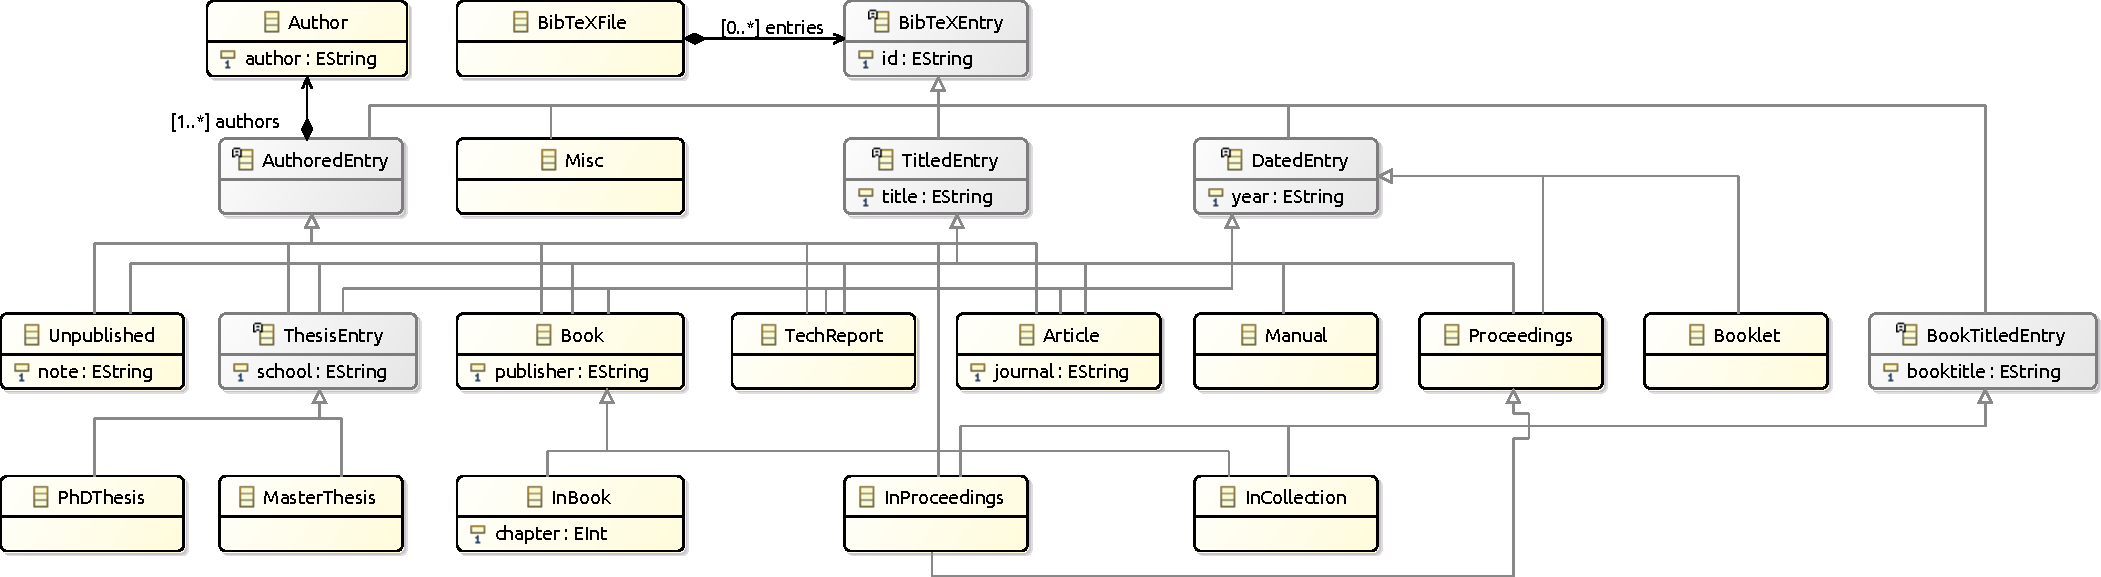
\includegraphics[width=\textwidth]{bibtex}
  \caption{Class diagram for the input BibTeXML metamodel}
  \label{fig:bibtex-mm}
\end{figure}

\begin{figure}
  \centering
  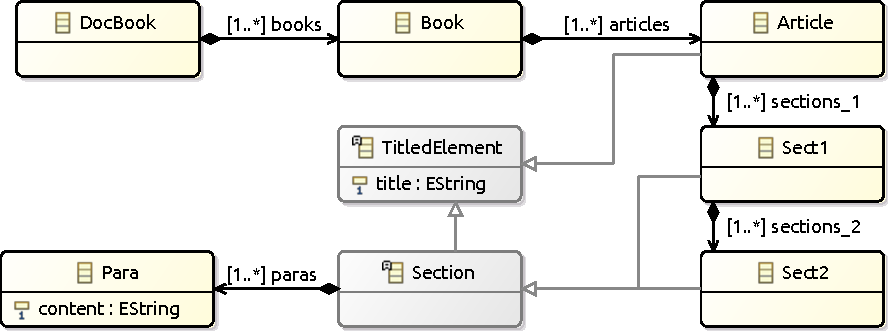
\includegraphics[width=.5\textwidth]{docbook}
  \caption{Class diagram for the target DocBook metamodel}
  \label{fig:docbook-mm}
\end{figure}

The rest of the document is structured as follows:
Section~\ref{sec:case-structure} describes the structure of the live case.
Section~\ref{sec:task-description} describes the proposed tasks for this live
case. Section~\ref{sec:benchmark-framework} mentions the benchmark framework for
those solutions that focus on raw performance. Finally,
Section~\ref{sec:evaluation} mentions an outline of the initial audience-based
evaluation across all solutions, and the approach that will be followed to
derive additional prizes depending on the attributes targeted by the solutions.

\section{Case Structure}
\label{sec:case-structure}

The case is intended to review the different approaches for checking
after-the-fact inter-model consistency between a BibTeX model and a DocBook
model. The process is roughly as follows:

\begin{enumerate}
\item The BibTeX model is generated randomly to a certain size, by the included
  \emph{generator} in the \file{models/generator.jar} JAR. The generator uses a
  Java port of the Ruby Faker\footnote{\url{https://github.com/DiUS/java-faker}}
  library to produce pseudorandom data given a seed. A number of random models
  (sizes 10, 100, 1000 and 10000) were generated in advance and included in the
  case resources.

\item The BibTeX model is transformed automatically to DocBook by the repackaged
  version of the original ATL transformation in the \file{bibtex2docbook.jar}
  JAR. This transformation deals well with models up to 1000 entries, but
  struggles with larger models due to recomputation of intermediate results.

\item The DocBook model is edited, in this case with the automated
  \emph{mutator} in the \file{models/mutator.jar} JAR. The mutator will operate
  on a DocBook file, creating a set of folders whose path will start with the
  specified prefix, adding \file{-N} from 1 to \file{nMutants}. Each folder will
  contain the mutated DocBook model, as well as a \emph{change model} explaining
  what was done to the model: Figure~\ref{fig:changes-mm} shows that such models
  have a \class{ModelChangeSet} as the root, with a number of
  \class{Model\-Change} instances of various types. The DocBook model will have
  gone through a number of random mutations according to a seed: if unspecified,
  the seed will be based on the current system time.

  \begin{figure}
    \centering
    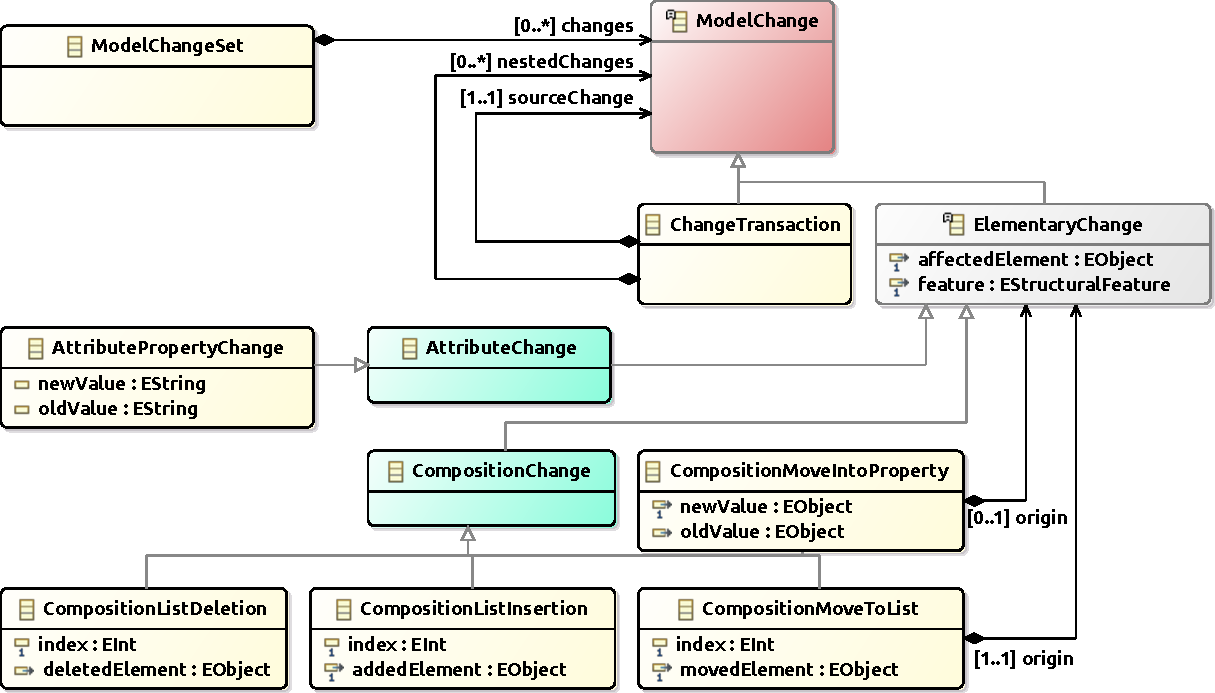
\includegraphics[width=.8\textwidth,keepaspectratio]{simplified-changes}
    \caption{Class diagram for the used subset of the Changes metamodel}
    \label{fig:changes-mm}
  \end{figure}

  The mutator has a number of predefined \emph{mutation operators} that will
  modify the model:

\begin{itemize}
\item Swapping paragraphs: this should break consistency in terms of sorting,
  but it will not result in missing information.
\item Swapping sections should not break consistency.
\item Deleting paragraphs/sections should break consistency.
\item Appending text to a paragraph should not break consistency.
\item Adding a new paragraph: unless it happens to match one of the authors,
  titles, or journals in its \class{Sect1}, it should not break consistency.
\end{itemize}

The mutated models were created in advance before the contest. There are three
sets of mutated models from the generated 10/100/1000-entry models: one with a
single mutation, one with two mutations, and one with three mutations.

\item A \emph{consistency checker} would take any combination of the previous
  artifacts (source BibTeX, fresh DocBook, mutated DocBook, change model) and
  make a judgment about whether the mutated DocBook is still consistent or not.

  If issues are found, it should point to the element in the source model which
  lacks a proper mapping on the other side, or the element in the target model
  which is not mapped correctly from the source model (e.g. it is not sorted
  anymore).

  The case resources include a set of expected results from the reference EVL
  consistency checker. However, the concrete definition of the consistency
  requirements has proven to be trickier to formalize than expected. This was
  raised by several case authors, and in fact one of the solutions considered
  creating a DSL for expressing inter-model consistency.
\end{enumerate}

\section{Task Description}
\label{sec:task-description}

The case had an optional and a mandatory task:

\begin{itemize}
\item The optional task was to re-implement or improve the original
  transformation itself, in a way that lent itself better to after-the-fact
  consistency checking. A transformation tool may have better support for this,
  or ATL could be made to deal better with larger versions of this model.

\item The mandatory task was to check for the consistency of the source BibTeX
  against the mutated DocBook models in the \file{models} directory, and report
  this information as efficiently and clearly as possible to the user. Ideally,
  this should be possible without a full re-run of the transformation. To be
  considered for the performance-related awards, solutions had to use the
  benchmarking framework in Section~\ref{sec:benchmark-framework}.
\end{itemize}

A reference solution based on the Epsilon Validation Language was provided. This
implementation did not re-run any transformations: instead, it did a two-way
consistency validation by checking from the BibTeX \class{BibTeXFile},
\class{Author}, \class{BibTeXEntry}, \class{TitledEntry}, and \class{Article}
types, and from the DocBook \class{Para} types. The implementation required 98
lines of EVL code and 113 lines of Java framework integration code, and does not
use the change models at all.

Solutions could focus on efficiency, conciseness, or clarity of presentation to
the user. Solutions that can operate straight from the definition of the
transformation (i.e.\ without a separate consistency checker) would be
preferred. The call for solutions also invited solution authors to consider
other desirable attributes, e.g. verifiability.

\section{Benchmark Framework}
\label{sec:benchmark-framework}

If focusing on performance, the solution authors had to integrate their solution
with the provided benchmark framework. It is based on the framework in the TTC
2017 Smart Grid case~\cite{hinkel_ttc_2017}, and supports the automated build
and execution of solutions. The benchmark consisted of three phases:

\begin{enumerate}
\item \textbf{Initialization}, which involved setting up the basic
  infrastructure (e.g. loading metamodels). These measurements are optional.
\item \textbf{Load}, which loaded the input models.
\item \textbf{Run}, which found the consistency violations in the mutated
  DocBook model.
\end{enumerate}

\subsection{Solution requirements}
\label{sec:solut-requ}

Each solution had to print to the standard output a line with the following
fields, separated by semicolons (``;''):

\begin{itemize}
\item \textbf{Tool}: name of the tool.
\item \textbf{MutantSet}: set of mutants used (``single'', ``double'' or ``triple'').
\item \textbf{Source}: base name of the input BibTeX model (e.g.\ ``random10.bibtex'').
\item \textbf{Mutant}: integer starting at 1, identifying the mutant model within this set.
\item \textbf{RunIndex}: index of the run of this combination of tools and inputs.
\item \textbf{PhaseName}: name of the phase being run.
\item \textbf{MetricName}: the name of the metric. It may be the used
  \textbf{Memory} in bytes, the wall clock \textbf{Time} spent in integer
  nanoseconds, or the number of consistency \textbf{Problems} found in the
  mutated DocBook model.
\end{itemize}

\lstinputlisting[
  float,frame=tb,numbers=left,
  caption={\file{solution.ini} file for the reference Epsilon solution},
  label=lst:ini-atl
]{../../solutions/Epsilon/solution.ini}

To enable automatic execution by the benchmark framework, solutions were in the
form of a subfolder within the \file{solutions} folder of the main
repository\footnote{\url{https://github.com/TransformationToolContest/ttc2019-live}},
with a \file{solution.ini} file stating how the solution should be built and how
it should be run. As an example, the \file{solution.ini} file for the reference
solution is shown on Listing~\ref{lst:ini-atl}. In the \file{build} section, the
\file{default} option specifies the command to build and test the solution, and
the \file{skipTests} option specifies the command to build the solution while
skipping unit tests. In the \file{run} section, the \file{cmd} option specifies
the command to run the solution.

The repetition of executions as defined in the benchmark configuration was done
by the benchmark. For 5 runs, the specified command will be called 5 times,
passing any required information (e.g. run index, or input model name) through
environment variables. Solutions could not save intermediate data between
different runs: each run had to be entirely independent.

The name and absolute path of the input model, the run index and the name of the
tool were passed using environment variables \file{Tool}, \file{MutantSet},
\file{SourcePath}, \file{Mutant}, \file{MutantPath}, and \file{RunIndex}.

\subsection{Running the benchmark}
\label{sec:running-benchmark}

The benchmark framework only required Python 3.3 to be installed. Solutions
could use any languages or frameworks, as long as they could run without human
input. Since all the performance-oriented solutions this year were compatible
with GNU/Linux, it was possible for the case authors to create a
\file{Dockerfile} with all solutions built in, for the sake of reproducibility.
The resulting image is available on Docker
Hub\footnote{\url{https://hub.docker.com/r/bluezio/ttc2019-live-git}}, and it is
automatically rebuilt on any push to the repository.

If all prerequisites are fulfilled, the benchmark can be run using Python with
the command \file{python scripts/run.py}. Additional options can be queried
using the option \file{{-}{-}help}. The benchmark framework can be configured
through the \file{config/config.json} file: this includes the input models to be
evaluated (some of which have been excluded by default due to their high cost
with the sample solution), the names of the tools to be run, the number of runs
per tool+model, and the timeout for each command in milliseconds.

\section{Evaluation}
\label{sec:evaluation}

The evaluation operated on several dimensions:

\begin{itemize}
\item How efficient was the approach in time and space (memory)? The reference
  ATL solution struggled with large models, and the reference solution was not
  been designed with performance in mind.

\item Was consistency checking directly supported by the transformation
  approach? Many tools lack this capability, though it might be interesting as
  an additional execution mode if the target model has seen manual changes since
  it was generated.

\item How informative and accessible was the feedback that can be provided by
  the approach?
\end{itemize}

Authors were invited to make submissions targeting other quality attributes. In
fact, one of the submissions targeted verifiability through formal methods.

\bibliographystyle{plain}
\bibliography{bibliography}

\end{document}
